\chapter{Описание решения} \label{ch2}

Код для построения одномерной геомеханической модели представлен по ссылке \cite{geomechanics_code}.
Структура кода соответствует описанным выше этапам построения геомеханической модели.

Первым шагом строятся планшеты для пластового давления и вертикального напряжения в зависимости от измеренной глубины (MD, measured depth) вдоль ствола скважины (рис. \ref{fig:geo1}).


\begin{figure}[H] 
	\center
	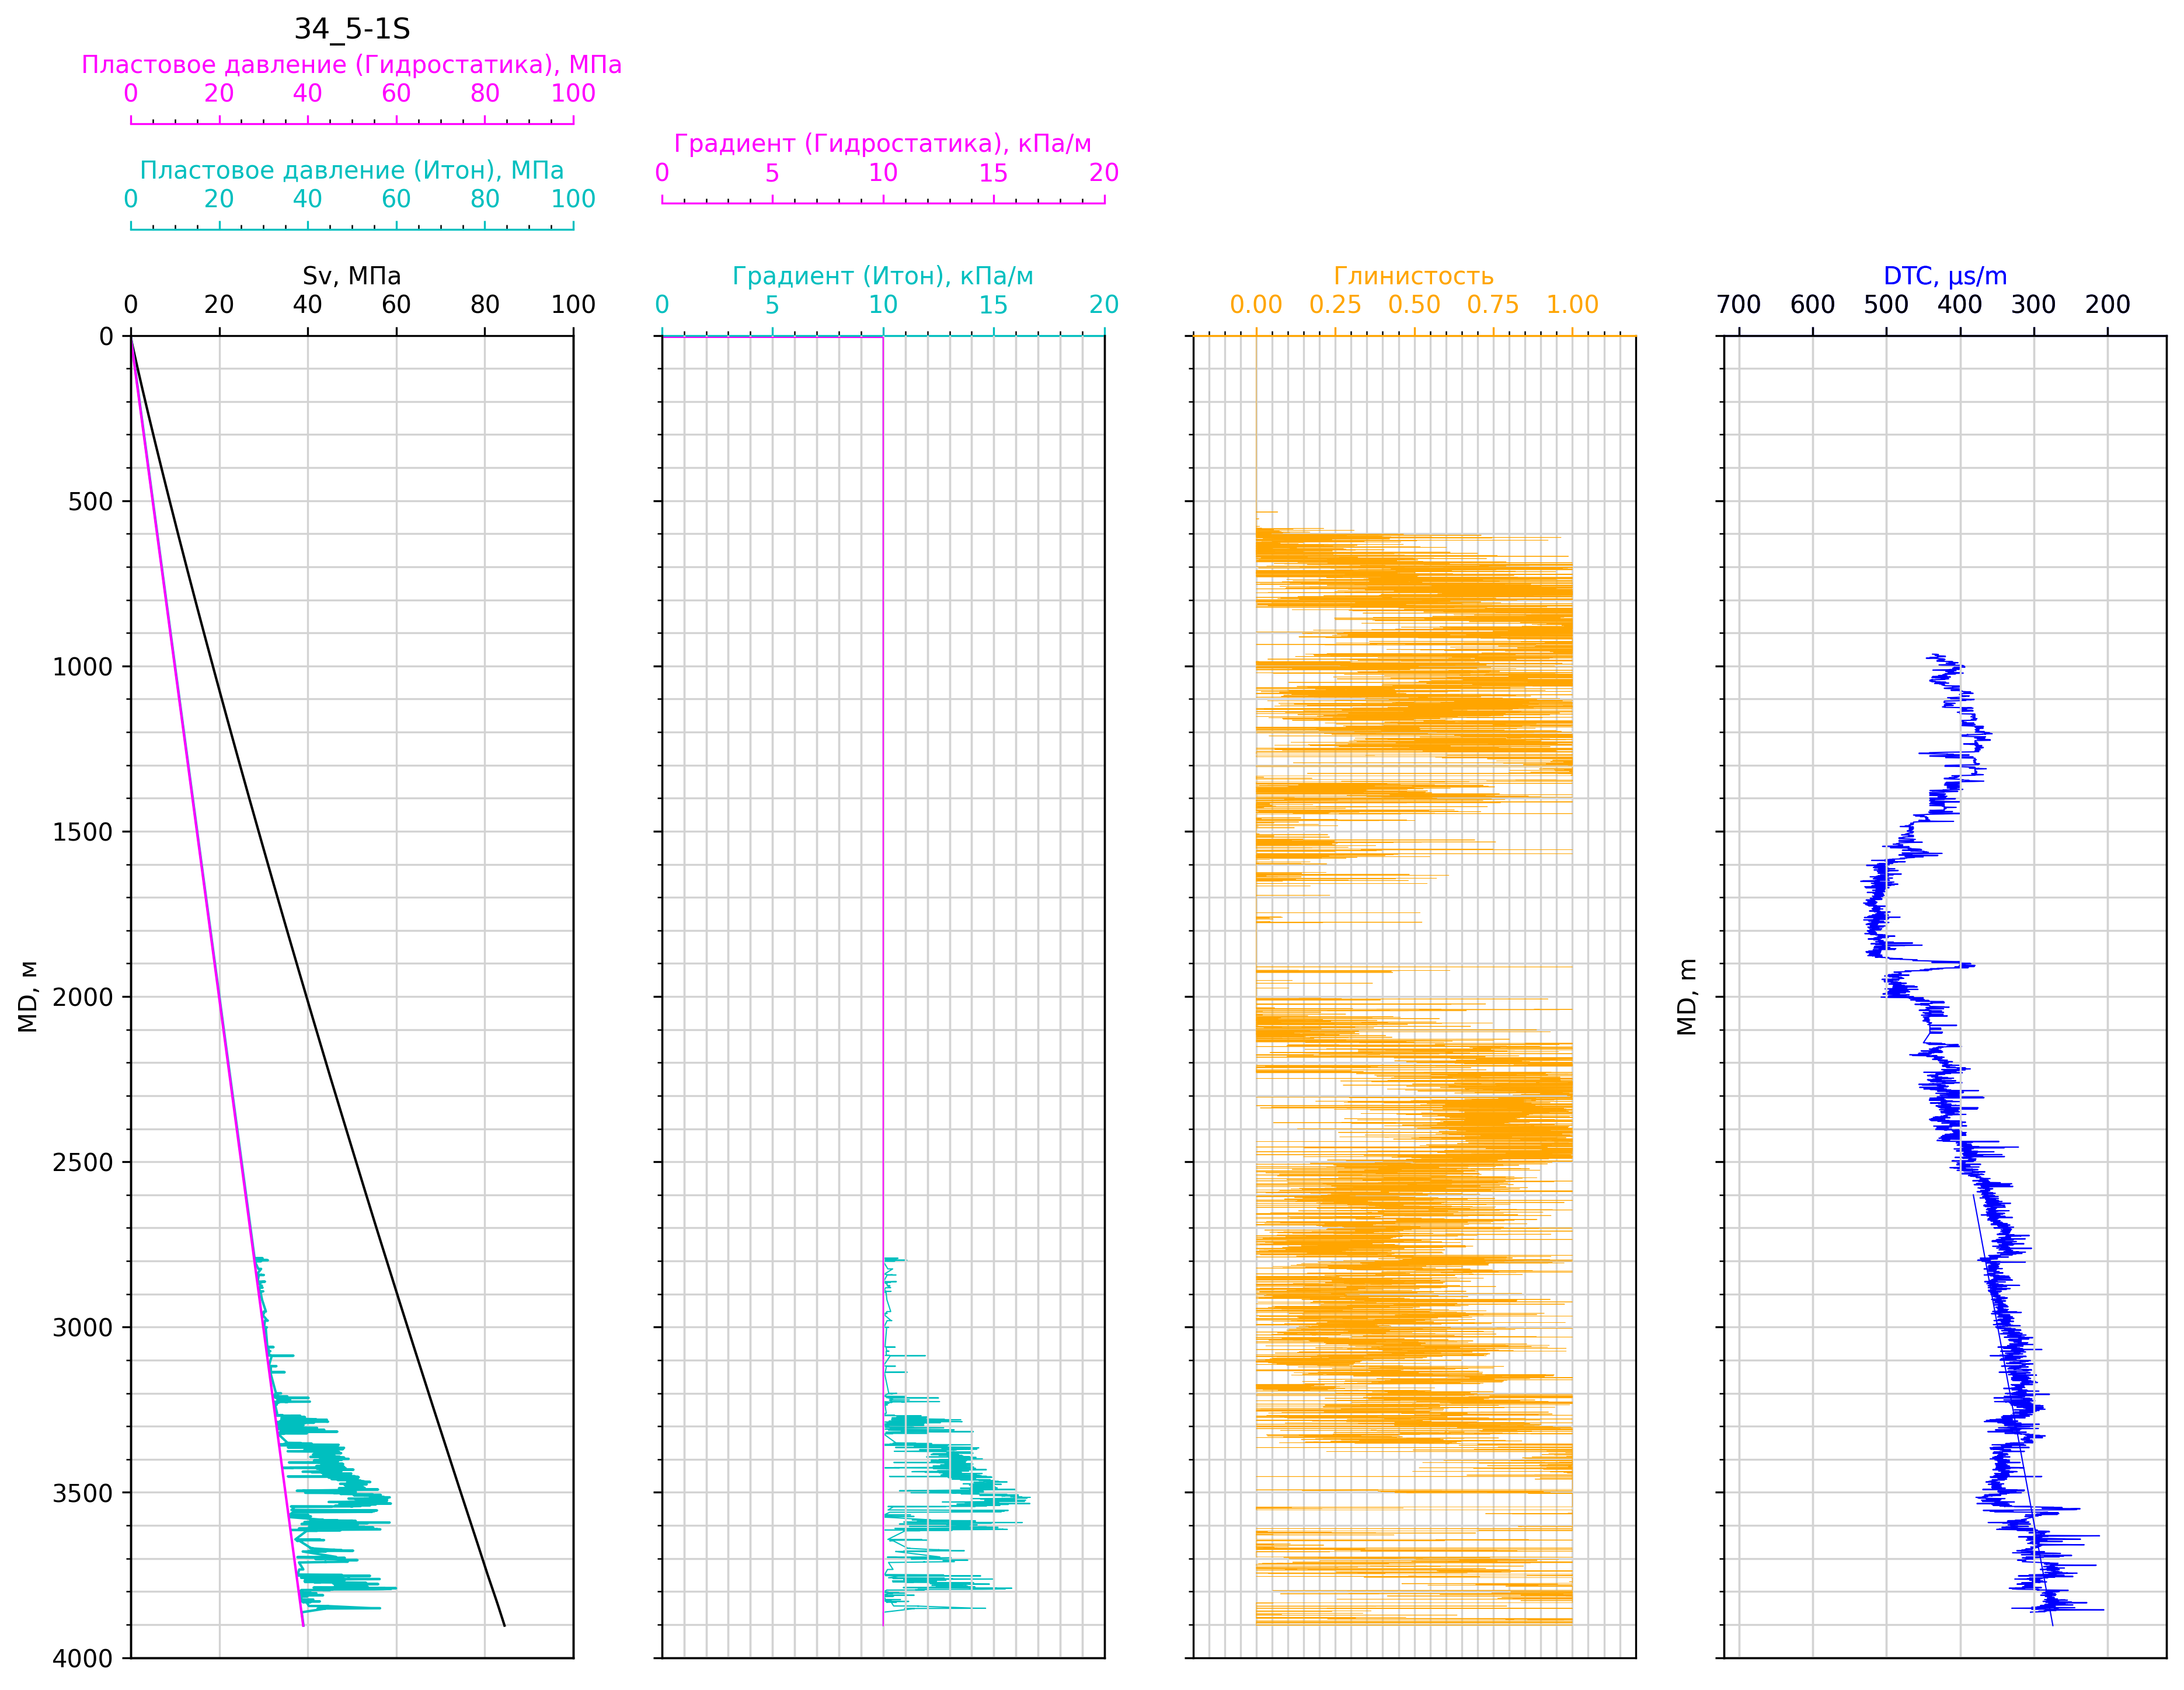
\includegraphics[width=.9\textwidth]{GeoMechanics1.png}
	\caption{Планшеты пластового давления и его градиентов (гидростатических и по Итону), планшеты глинистости и кросс-дипольного каротажа}
	\label{fig:geo1}
\end{figure}

Далее на основе данных широкополостного акустического каротажа и кросс-дипольного каротажа определяются динамические упругие модули породы.
Затем на основе имеющихся керновых данных строятся корреляции между статическими и динамическими упругими модулями породы.

Полученные профили статических и динамических упругих модулей отображены на графиках в зависимости от измеренной глубины (MD) вдоль ствола рассматриваемой скважины (рис. \ref{fig:geo2}).

\begin{figure}[H] 
	\center
	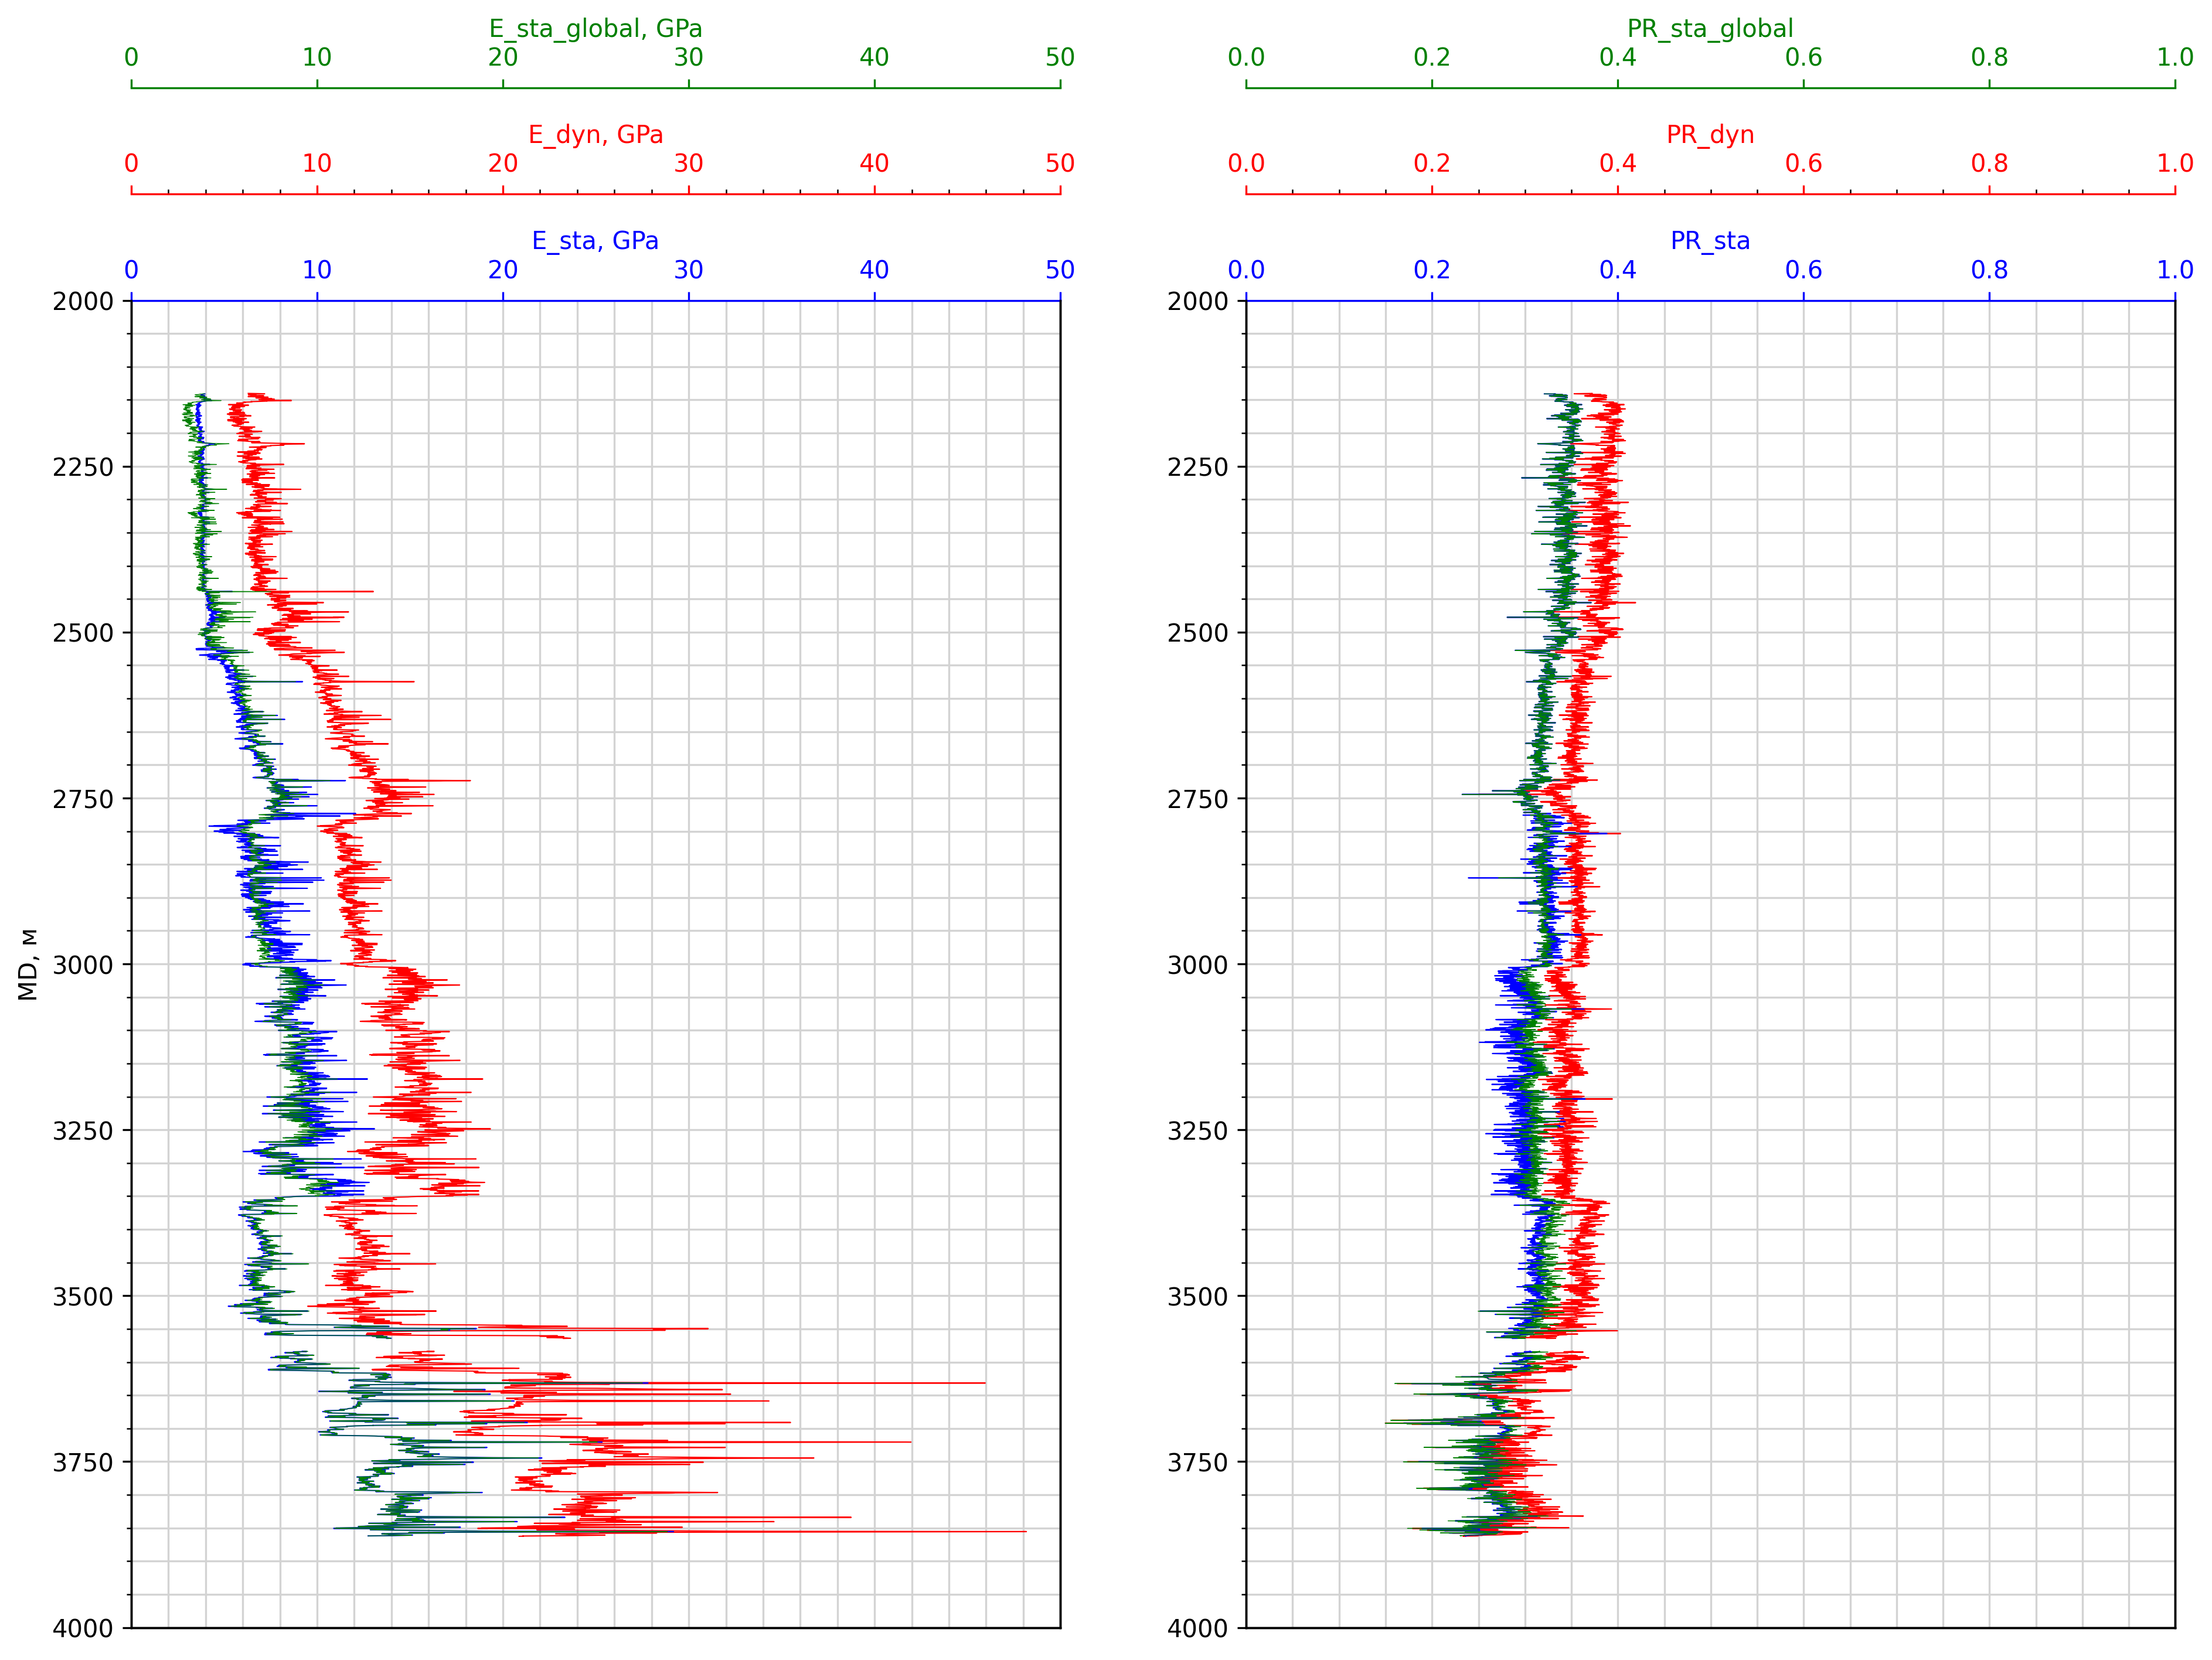
\includegraphics[width=.9\textwidth]{GeoMechanics2.png}
	\caption{Планшеты статических и динамических модулей Юнга и коэффициентов Пуассона вдоль скважины}
	\label{fig:geo2}
\end{figure}

Для каждого упругого модуля на графиках представлено по 3 профиля: динамический (получен на основе данных акустического каротажа), статический (найден по корреляциям по пяти зонам – каждая из зон определена вручную по единообразному тренду) и глобальный статический (найден по глобальной корреляции между всеми керновыми данными и соответствующими по глубине данными ГИС).

\begin{figure}[H] 
	\center
	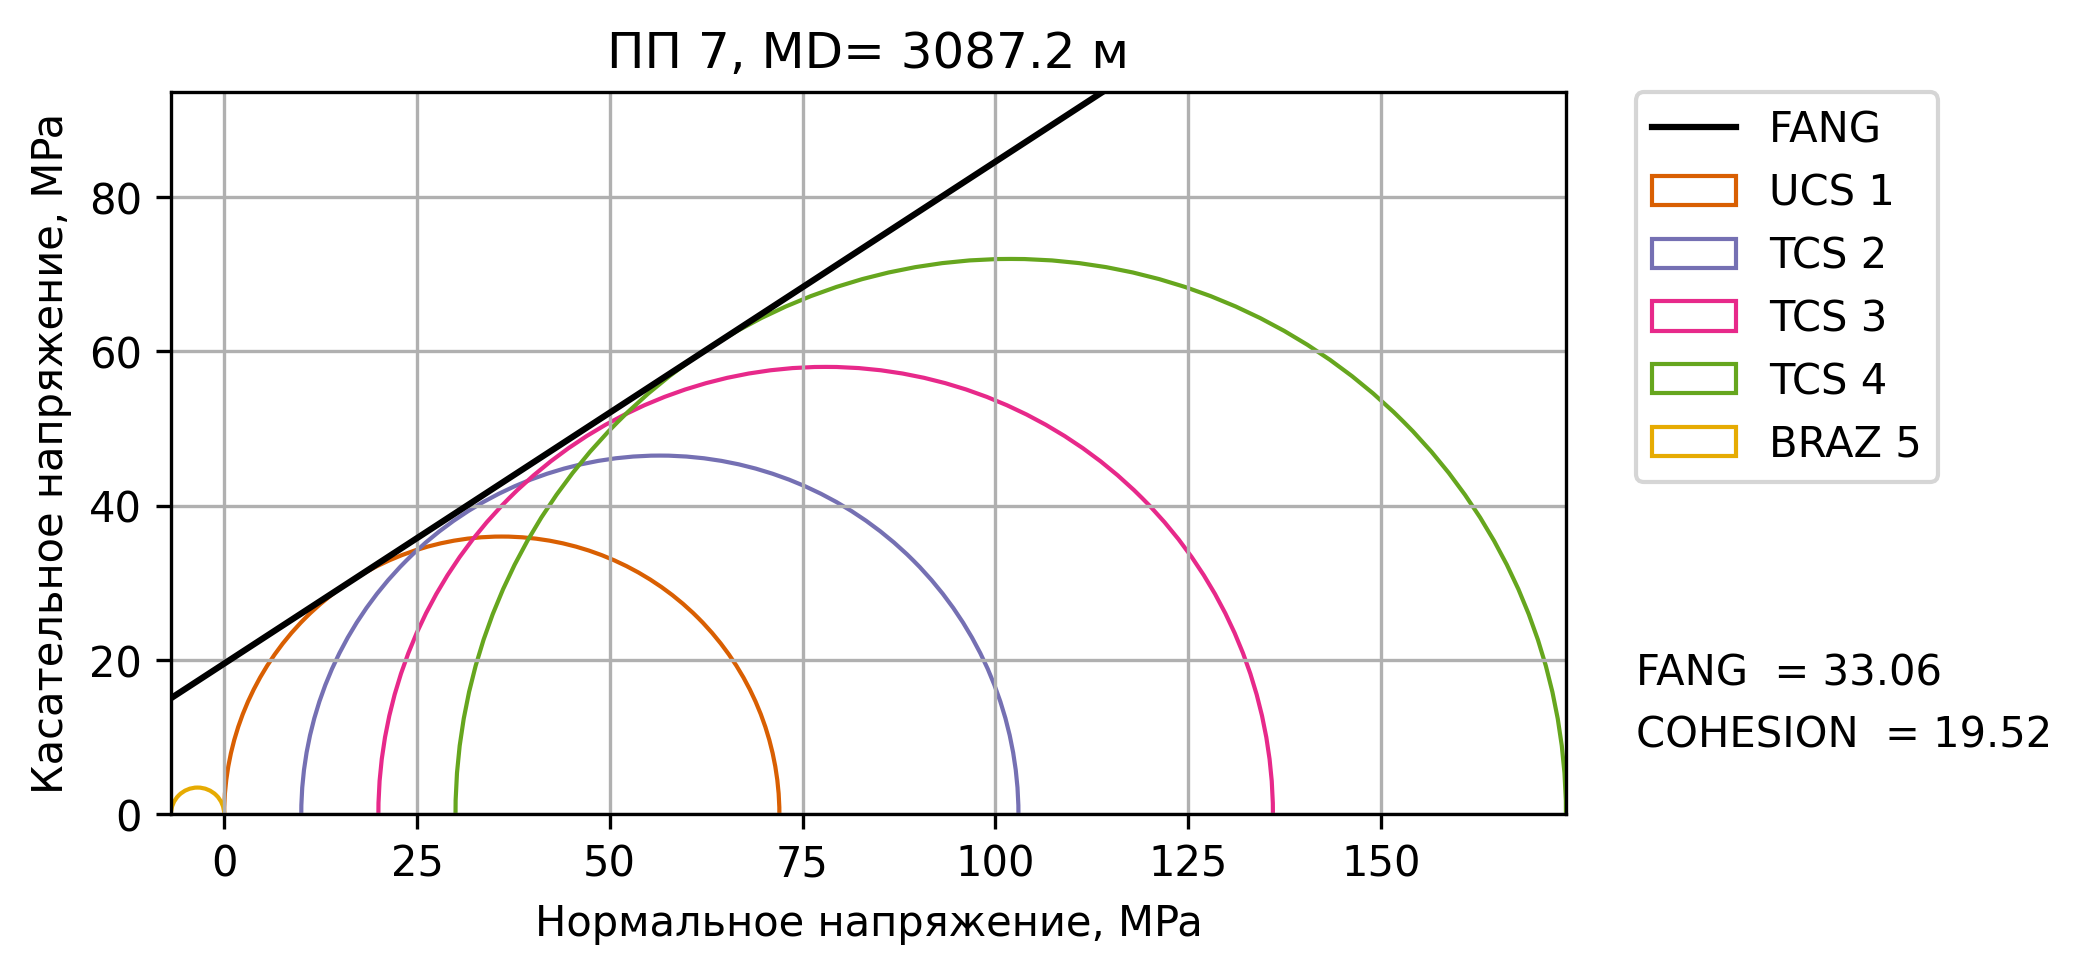
\includegraphics[width=.8\textwidth]{GeoMechanics3.png}
	\caption{Паспорт прочности для образца керна, отобранного с глубины $MD=3087.2\text{ м}$}
	\label{fig:geo3}
\end{figure}

Далее на основе экспериментов над каждым из образцов керна строятся паспорта прочностных свойств каждого из них. На рис. \ref{fig:geo3} представлен пример построенного паспорта прочности для одного из образцов керна.

Затем производится расчёт горизонтальных напряжений по пороупругой модели и строится финальный планшет градиентов и напряжений (рис. \ref{fig:geo4}).
На этом планшете отображаются градиент пластового давления, градиент обвала (равен плотность бурового раствора, ниже которой ствол скважины будет обваливаться), градиент начала поглощений бурового раствора, градиент ГРП (градиент разрыва породы), а также профили пластового давления, минимального и максимального главных горизонтальных напряжений, главного вертикального напряжения.

По полученному итоговому планшету (см. рис. \ref{fig:geo4}) можем сделать вывод, что рассматриваемая вертикальная скважина очень устойчива, так как градиент обвала существенно ниже градиента пластового давления.

\begin{figure}[H] 
	\center
	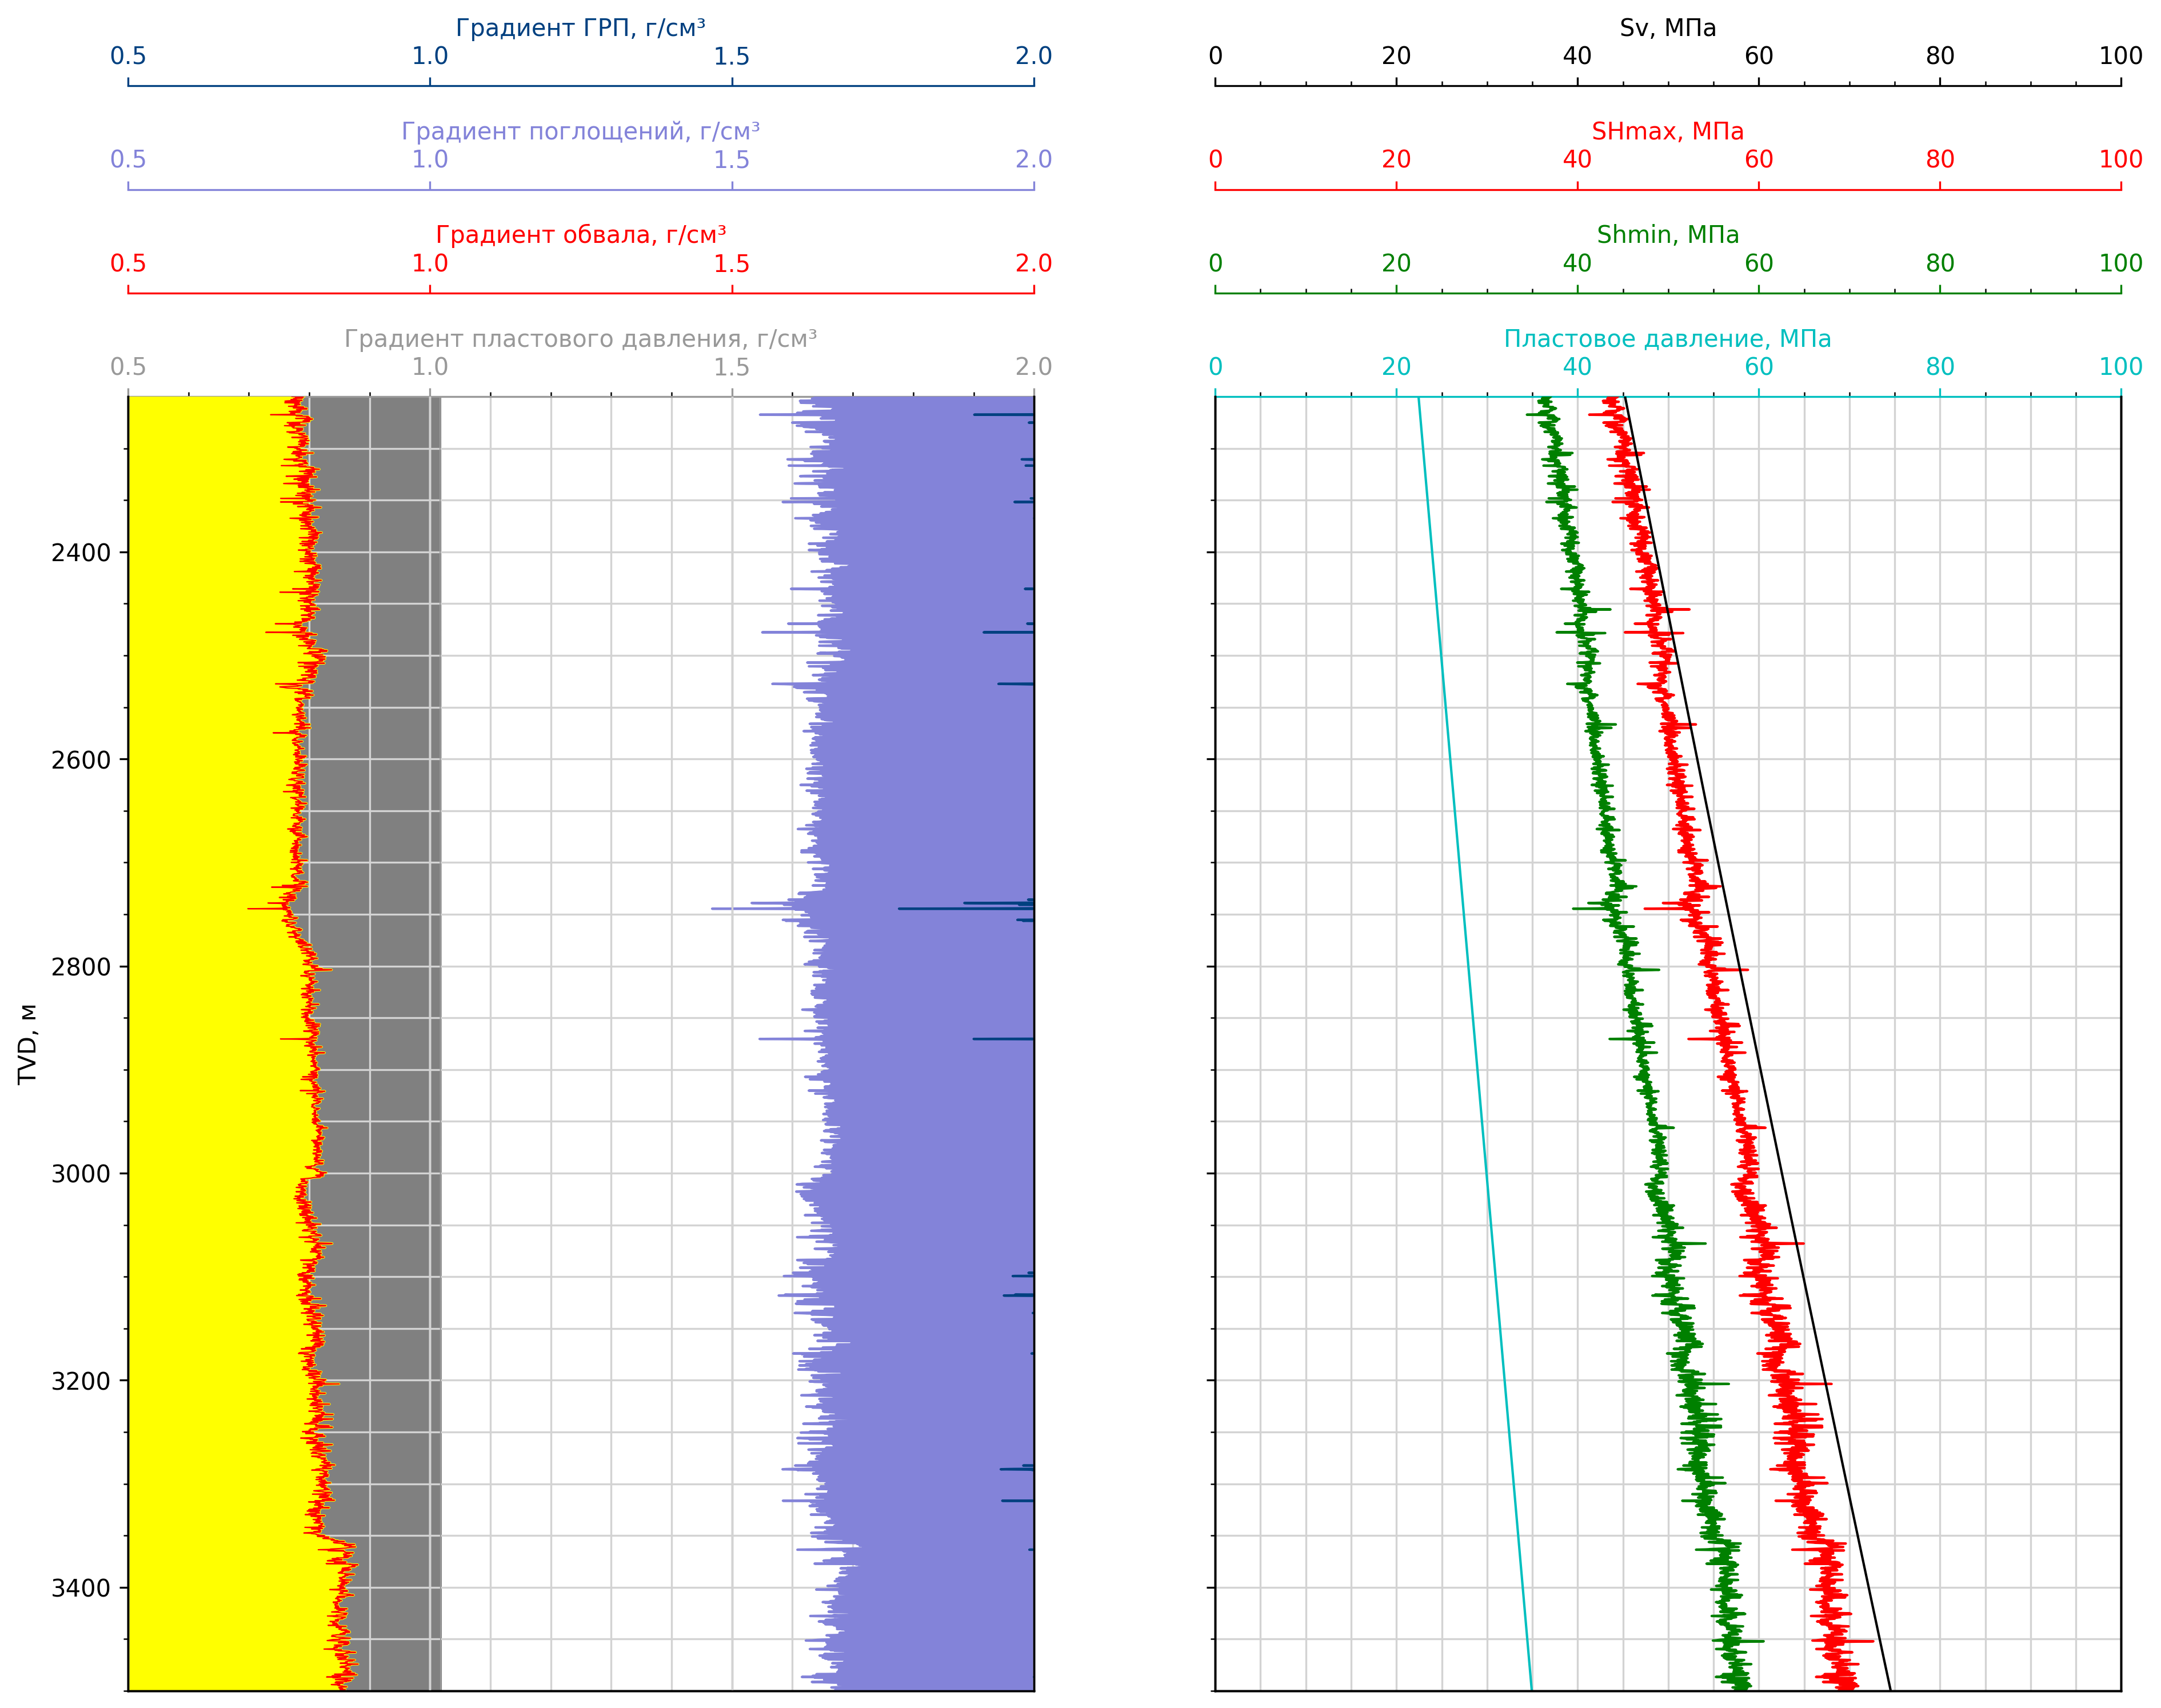
\includegraphics[width=.9\textwidth]{GeoMechanics4.png}
	\caption{Планшет градиентов и напряжений вдоль ствола скважины
(построен по истинной вертикальной глубине TVD)}
	\label{fig:geo4}
\end{figure}

%\section{Название параграфа} \label{ch2:sec1}


